\label{section:methods}

This work uses a multicomponent Lattice Boltzmann Method (LBM) to simulate the hydrodynamics of two partially miscible, 
incompressible fluids as implemented in LB3D. The LBM solves the Navier-Stokes equation at the incompressible limit, 
$\rho \frac{d \overrightarrow{u}}{dt} = \eta \Delta \overrightarrow{u} + \frac{\nabla P}{\rho} + F_{body}$, at low 
Mach and Reynolds numbers, incorporating density $(\rho)$, viscosity $(\eta)$, velocity $(u)$, pressure $(P)$, and 
body force $(F_{body})$. \cite{qian_lattice_1992, chin_lattice_2002, nourgaliev_lattice_2003} The Shan-Chen pseudopotential
model is used to simulate the Cahn-Hilliard equation, $\frac{d c^k}{dt} = M^k\Delta \mu - \nabla u^k c^k$, for the non-ideal 
mixture model. \cite{shan_lattice_1993, shan_simulation_1994, he_lattice_1997, he_discrete_1998} $c^k$, $M^k$ and $u^k$ is the 
concentration, mobility and velocity of species $k$ respectively while $\mu$ is the free energy of system. Particle dynamics 
include Hertzian contact and lubrication forces, tracked with classical Newtonian mechanics, while particle-fluid coupling 
involves momentum exchange to simulate viscous dissipation. Particle-particle magnetic interactions are modeled using dipole 
interactions. \cite{davies_interface_2014, xie_direct_2017, xie_controllable_2021} A more detailed description of the model is 
provided in the following sections

\section{Hydrodynamics} 
\label{section:lbm_hydrodynamics}

The lattice boltzmann method works by evolving a population distribution $f_{i}(\mathbf{x}, t)$ on a cubic lattice with 
timestep $\Delta t$ with lengthscale $\Delta x$. \cite{qian_lattice_1992, succi_lattice_2018, he_theory_1997} The D3Q19 
velocity set is used in this work with the indexes $i$ represent each of the 19 velocities and converves mass and momentum 
conservation to the second order. It can be seen in Figure \ref{fig:d3q19_lattice}. The algorithm is split into the 
collision step where the populations on each lattice grid cell are relaxed towards an equilibrium, followed by the 
advection step where populations in each velocity direction are propagated with velocity $\mathbf{c_i}$. 

The collision step occurs using a single relaxation time Bhatnagar-Gross-Krook (BGK) collision operator at relaxation 
rate $\tau$. \cite{bhatnagar_model_1954, qian_lattice_1992} The combined collision and advection LBM is expressed below 
in equation \ref{eq:LBM_BGK}

\begin{equation}
    f_{i}(\mathbf{x} + \mathbf{c}_{i}\Delta t, t + \Delta t) = f_{i}(\mathbf{x}, t) - \frac{1}{\tau}(f_{i}(\mathbf{x}, t) 
    - f_{i}^{eq}(\mathbf{x}, t))
    \label{eq:LBM_BGK}
\end{equation}

The BGK operator limits simulations to low reynolds number and mach numbers to prevent numerical instabilities. 
\cite{qian_lattice_1992} The kinematic viscosity if using the BGK operator is defined as 
$\nu = c_s^2(\tau - \frac{\Delta t}{2})$. The equilibrium distribution is obtained from a discretized expansion of the 
Maxwell-Boltzmann distribution to the second order. \cite{he_theory_1997, succi_lattice_2018} This is shown in equation 
\ref{eq:LBM_Feq}.

\begin{equation}
    f_{i}^{eq}(\mathbf{x}, t) = w_i\rho(1 + \frac{\mathbf{c_i} \cdot \mathbf{u}}{c_s^2} + \frac{(\mathbf{c_i} \cdot 
    \mathbf{u})^2}{2c_s^4} + \frac{\mathbf{u} \cdot \mathbf{u}}{2c_s^2} + \frac{(\mathbf{c_i} \cdot 
    \mathbf{u})^3}{6c_s^6} - \frac{(\mathbf{c_i} \cdot \mathbf{u})\mathbf{u}^2}{4c_s^3})
    \label{eq:LBM_Feq}
\end{equation}

\begin{figure}[h]
    \centering
    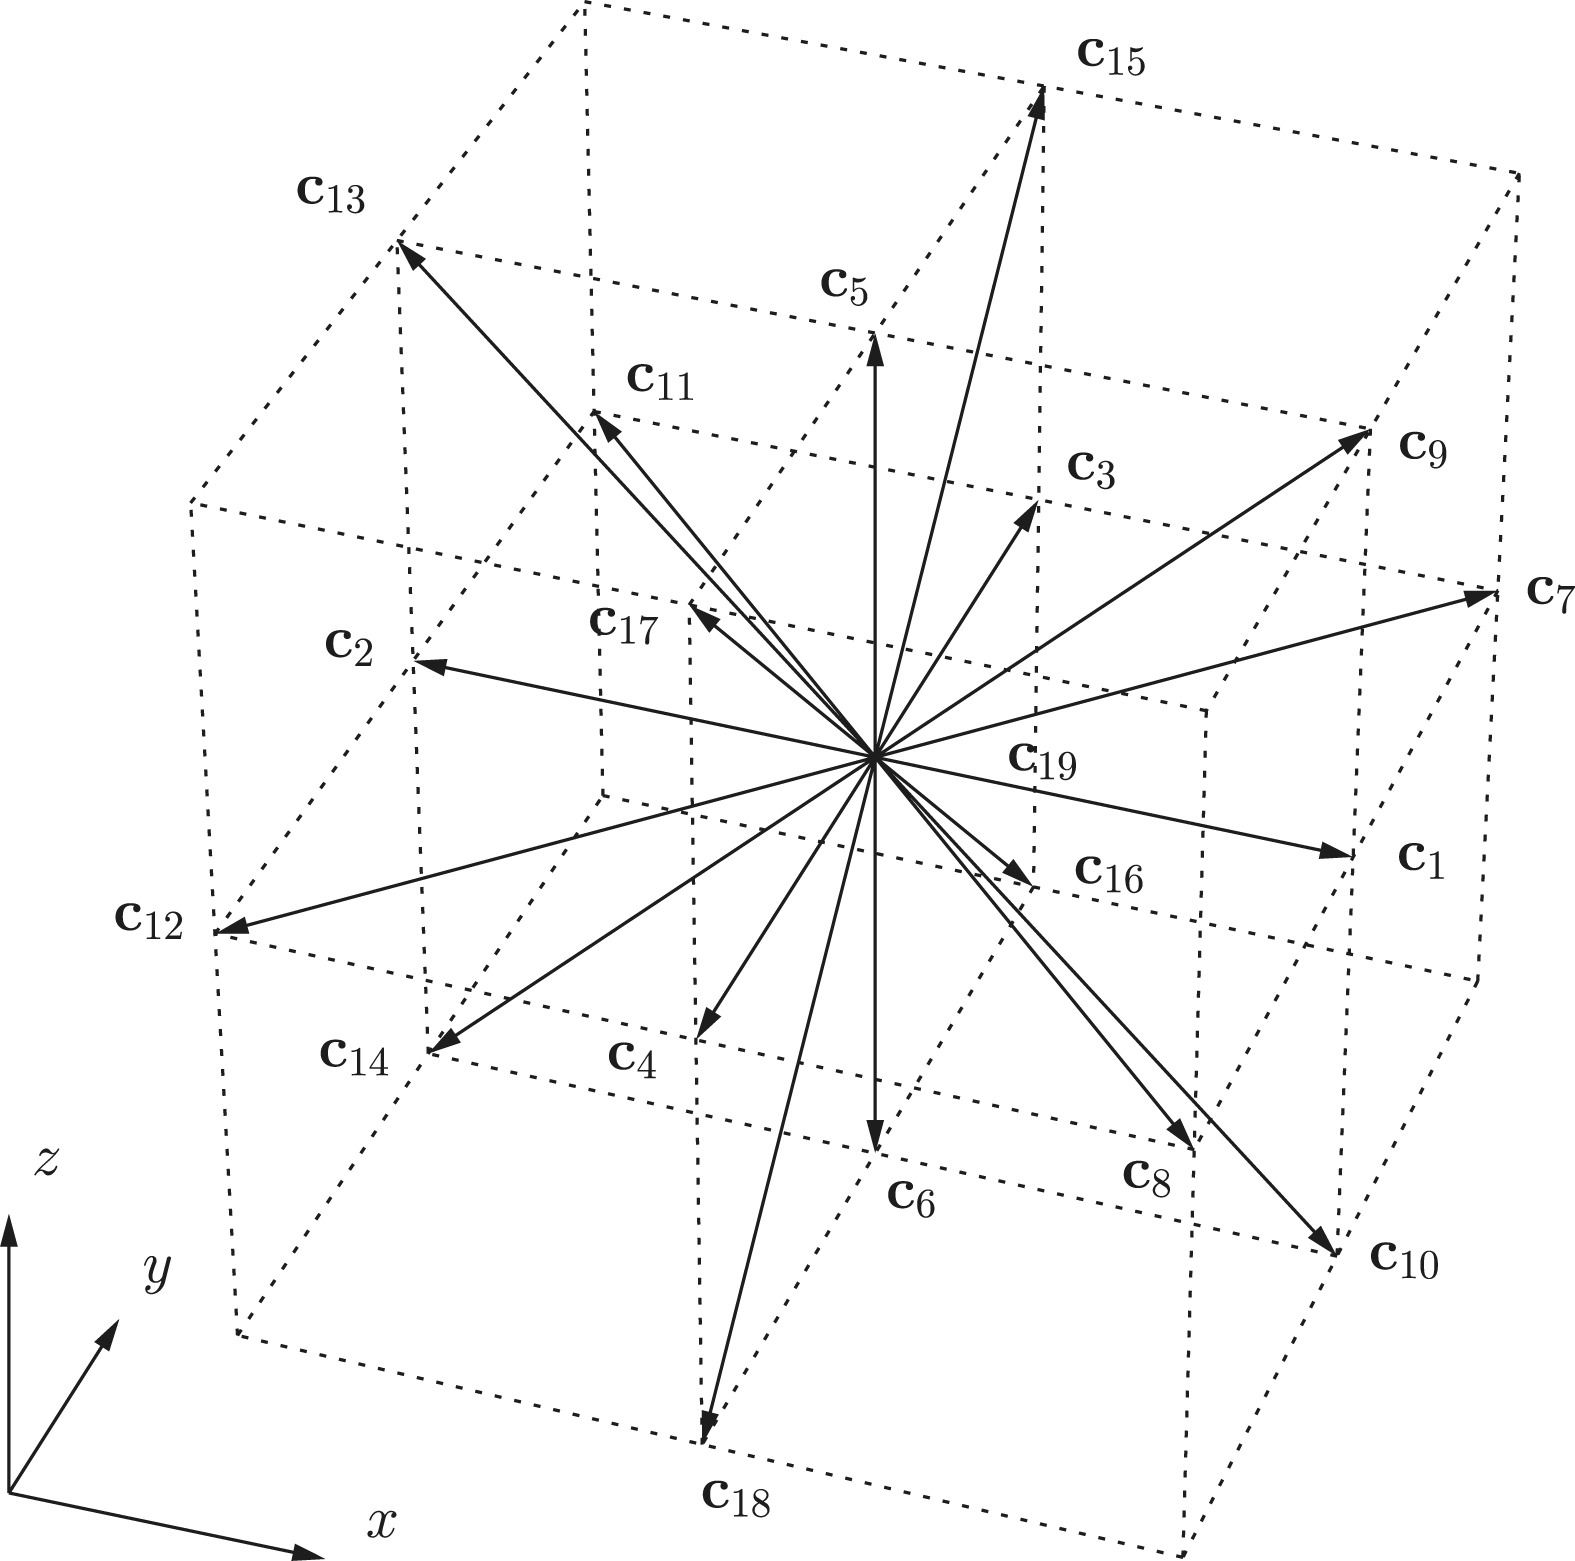
\includegraphics[scale = 0.7]{figures/methods/d3q19_lattice.jpg}
    \caption{D3Q19 lattice demonstrating the rest, nearest and next nearest direction that correspond to the 19 
    directions $(i)$ of the lattice with lattice velocity $c_{i}$. \cite{schmieschek_lb3d_2017} Reproduced from 
    Schmieschek et al. under the Creative Commons license.}
    \label{fig:d3q19_lattice}
\end{figure}

$\rho$ and $\textbf{u}$ in Equation \ref{eq:LBM_Feq} are defined as the macroscopic parameters for density and velocity 
and can be calculated from the mass distribution using $\rho = \sum f_i$ and $\rho \mathbf{u} = \sum f_i \mathbf{c}_i$ 
respectively. Using the Chapman-Enskog expansion, the Navier-Stokes equation at the incompressible limit at low-reynolds 
numbers can be recovered. \cite{qian_lattice_1992, he_lattice_1997} The regime accessible through this method is suitable 
for simulations in this work as the $ 1 \leq Re \leq 100 $ and the mach number, $Ma < 0.01$, fulfilling the stability 
criterion and usage requirements for the presented hydrodynamic model.

\section{Non-ideal mixing}
\label{section:lbm_hydrodynamics}

The SC model mimics Cahn-Hilliard type behaviour through a force applied from the other fluid species $k'$ in adjacent 
cells $\mathbf{x'}$ on fluid species $k$ at point $\mathbf{x}$. \cite{shan_lattice_1993, shan_simulation_1994, 
shan_multicomponent_1995, he_discrete_1998, jansen_bijels_2011, chin_lattice_2002} Both fluid species are defined
 by their own distribution equation defined in Equation \ref{eq:LBM_BGK} The strength of this force is controlled 
 through an interaction parameter, $g_{kk'}$ with no contribution from self interaction of the fluid as these are 
 set to zero. The SC force can then be written out in Equation \ref{eq:sc_model}.

\begin{equation}
F_{k}^{SC}(\mathbf{x}, t) = -\Psi^{k}(\mathbf{x}, t)\sum_{k'}g_{cc'}\sum_{\mathbf{x'}}\Psi_{k'}(\mathbf{x'}, t)(\mathbf{x'} 
- \mathbf{x})
\label{eq:sc_model}
\end{equation}

An effective mass of each fluid at node $\mathbf{x}$ is used in place of the actual density to scale it between zero 
and one and is defined as $\psi^{c}(\mathbf{x},t) = \rho_{0}\left[1 - \exp(-\frac{\rho^{k}(\mathbf{x}, t)}{\rho_{0}})\right]$. 
In this model, the SC force is incorporated into the macroscopic velocities written as 
$\mathbf{u}_k =  \mathbf{u}_k + \frac{\tau}{\rho} F_{k}$ and finally the equilibrium distribution of each fluid species. 

\section{Suspended particle dynamics}
\label{section:lbm_colloids}

Suspended particles will be coupled to the LB fluid based on the work conducted by Ladd. \cite{ladd_numerical_1994, 
aidun_direct_1998, ladd_lattice-boltzmann_2001} The particles follow Newtonian mechanics with force 
$\mathbf{F_p} = m_p\frac{d \mathbf{u_p} }{dt}$ and rotational inertia $\mathbf{D_p} = J_p \frac{d \mathbf{\omega_{p}}}{dt}$. 
$\mathbf{F_p}$ and $\mathbf{D_p}$ represent the force and torque acting on a particle with mass $m_p$ and moment of inertia 
$J_p$. $\mathbf{u}_p$ and $\mathbf{\omega_{p}}$ are the linear and angular velocities of the particle. The equations of 
motion are evolved over time using a leapfrog integrator. \cite{jansen_bijels_2011}

The particles are discretized on the lattice according to the method laid out in Ladd and Aidun 
\cite{ladd_lattice-boltzmann_2001}. Coupling to the LB fluid is done through momentum exchange with the 
fluid through modification of the velocity surrounding the fluid. The discretized particles have a no-slip 
boundary condition implemented as a modified bounce back boundary condition, with momentum exchange between 
particle and fluid done by changing the post collision population distribution, $f^{*}_{i}(\mathbf{x}, t)$, 
shown in Eq \ref{eq:md_LBM_mod}

\begin{equation}
    f^{*}_{i'}(\mathbf{x}, t + \Delta t) = f^{*}_{i}(\mathbf{x}, t) - \frac{2 w_{i}}{c_s^2}\rho^k \mathbf{u}_{surf} 
    \cdot \mathbf{c_i}
    \label{eq:md_LBM_mod}
\end{equation}

In this work, $i'$ is defined such that $\mathbf{c_i} = -\mathbf{c_{i'}}$ to satisfy the bounce-back boundary condition. 
The fluid velocity at the particle surface, $\mathbf{u}_{surf}$, is the sum of the particle's linear and rotational 
velocities, $\mathbf{u}_{surf} = \mathbf{u_p} + R_i\mathbf{\omega_p}$. Advection of populations occurs after this exchange. 
The total force and torque on the particle are calculated by summing the total momentum over its surface. As particles 
move, they cover and uncover fluid grid points. Covered points are removed, while the composition of newly uncovered 
points in a multiphase fluid is averaged from adjacent grid points. 

\subsection{Anisotropic particles}
\label{section:lbm_colloids_ellipsoids}

Under 1 lattice unit additional lubrication forces are required to reduce the likelihood of particle overlap. For 
spherical particles, this is defined in Equation \ref{eq:sphere_lube}

\begin{equation}
    \mathbf{F}_l = -6\pi \eta \frac{R_{i}^{2} R_{j}^{2}}{(R_i + R_j)^2}(\frac{1}{|\mathbf{r}_{ij}| -R_i - R_j} -\frac{1}{\Delta_c}) \frac{(\mathbf{u}_{ij}\cdot\mathbf{r}_{ij})\mathbf{r}_{ij}}{|\mathbf{r}_{ij}|^2}
    \label{eq:sphere_lube}
\end{equation}

where $R_i$ and $R_j$ are the radii of each particle involved in the interaction, $\mathbf{r}_{ij}$ is the distance
 vector between the particle centers, $\mathbf{u}_{ij}$ are the relative velocities of the particles and $\Delta_c$ 
 is the cutoff distance when the lubrication force begins to act. A hertzian contact force is also added to ensure 
 that there is no particle overlap, defined in Equation \ref{eq:hertz_def}

\begin{equation}
    \phi_{H} = K_{H}(R_i + R_j - |\mathbf{r}_{ij}|)^{5/2}, r < R_i + R_j
    \label{eq:hertz_def}
\end{equation}

$K_H$ is the force constant used to push particles apart. To correct for the anisotropic particles used in this work, 
the formulas presented in Eqs \ref{eq:sphere_lube} and \ref{eq:hertz_def} can be generalized using the route followed 
in Gunther et al. and Davies et al., inspired by Berne and Pechukas. \cite{gunther_timescales_2014, davies_interface_2014} 
They first begin by rewriting the lubrication and Hertzian contact forces in a dimensionless form below

\begin{equation}
    \phi_{H}(\hat{\mathbf{o_i}}, \hat{\mathbf{o_j}}, \hat{\mathbf{r_{ij}}}) = \epsilon(\hat{\mathbf{o_i}}, 
    \hat{\mathbf{o_j}})\Bar{\phi_{H}}\left( \frac{r_{ij}}{\sigma(\hat{\mathbf{o_i}}, \hat{\mathbf{o_j}}, 
    \hat{\mathbf{r_{ij}}})} \right)
    \label{eq:hertz_anisotropic}
\end{equation}

Equation \ref{eq:hertz_anisotropic} defines the generalization of the Hertz force to allow simulation of ellipsoidal 
particles inspired by Berne and Pechukas. First, the hertzian force is made a function of orientation through the 
addition of eccentricity, $\chi = \frac{R_p^2 - R_o^2}{R_p^2 + R_o^2}$ and an orientation dependent forces, where 
$\epsilon(\hat{\mathbf{o_i}}, \hat{\mathbf{o_j}}) = \frac{\Bar{\epsilon}}{\sqrt{1 - \chi(\hat{\mathbf{o_i}}, 
\hat{\mathbf{o_j}})^2}}$, and $\sigma = \frac{\Bar{\sigma}}{\sqrt{1 - \frac{\chi}{2}( 
\frac{(\hat{\mathbf{r_{ij}}}\hat{\mathbf{o_i}} +  \hat{\mathbf{r_{ij}}}\hat{\mathbf{o_j}})^2}{1 + 
\chi \hat{\mathbf{o_i}}\hat{\mathbf{o_j}}} +  \frac{(\hat{\mathbf{r_{ij}}}\hat{\mathbf{o_i}} -  
\hat{\mathbf{r_{ij}}}\hat{\mathbf{o_j}})^2}{1 - \chi \hat{\mathbf{o_i}}\hat{\mathbf{o_j}}})}}$, 
$\Bar{\sigma} = 2R_{\perp}$. \cite{gunther_lattice_2013, gunther_timescales_2014, davies_assembling_2014}

A similar generalization process is done for the lubrication force, resulting in Equation \ref{eq:md_force} where 
$\mathbf{\Bar{F}}(r) = \hat{\mathbf{r_{ij}}}(\hat{\mathbf{r_{ij}}}(\mathbf{u}_i - \mathbf{u}_j))\left( \frac{1}{r - 1} - 
\frac{\sigma}{\Delta_{c}} \right)$. 

\begin{equation}
    \mathbf{F_{ij}}(\hat{\mathbf{o_i}}, \hat{\mathbf{o_j}}, \hat{\mathbf{r_{ij}}}) = \epsilon(\hat{\mathbf{o_i}}, 
    \hat{\mathbf{o_j}})\mathbf{\mathbf{F_{ij}}}\left( \frac{r_{ij}}{\sigma(\hat{\mathbf{o_i}}, \hat{\mathbf{o_j}}, 
    \hat{\mathbf{r_{ij}}})} \right)
    \label{eq:md_force}
\end{equation}

\subsection{Magnetic field and particle coupling}
\label{section:lbm_colloids_magnetics}

The magnetic dipole potential is defined as

\begin{equation}
    \mathbf{U_{ij}} = \frac{\mu_0 m_i m_j}{4\pi r_{ij}^{3}} \left[ \Hat{\mathbf{o_i}} \cdot \Hat{\mathbf{o_j}} - 
    3(\Hat{\mathbf{o_i}} \cdot \Hat{\mathbf{r_{ij}}})(\Hat{\mathbf{o_j}} \cdot \Hat{\mathbf{r_{ij}}}) \right]
    \label{eq:magnet_potential}
\end{equation}

Where $\mu_0 = 4\pi \cdot 10^{-7} \frac{H}{m}$,  $\Hat{\mathbf{o_i}}$ is the orientation unit vector of particle 
$i$, $\Hat{\mathbf{r_{ij}}}$ is the distance vector between particles $i$ and $j$ and $m_i$ is the magnitude the 
magnetic dipole of particle $i$. From the potential, the force and torque of the dipole force between particles 
can be found. These expressions are shown in equations \ref{eq:dipole_magnetic_force} and \ref{eq:dipole_magnetic_torque} 
for the force and torque respectively.

\begin{equation}
    \mathbf{F}_{ij} = \frac{3 \mu_0}{4 \pi} [\frac{5(m_i \cdot \mathbf{r}_{ij})(m_j 
    \cdot \mathbf{r}_{ij})}{|\mathbf{r}_{ij}|^7}\mathbf{r}_{ij} - \frac{(m_i \cdot m_{j})\mathbf{r}_{ij} + 
    (m_i \cdot \mathbf{r}_{ij})m_i + (m_j \cdot \mathbf{r}_{ij})m_j }{|\mathbf{r}_{ij}|^5}]
\label{eq:dipole_magnetic_force}
\end{equation}

\begin{equation}
    \mathbf{T}_{ij} = \frac{\mu_0}{4 \pi}[ \frac{3(m_j \cdot \mathbf{r}_{ij})m_i \times \mathbf{r}_{ij} }
    {|\mathbf{r}_{ij}|^5} - \frac{m_i \cdot m_j }{|\mathbf{r}_{ij}|^3} ]
    \label{eq:dipole_magnetic_torque}
\end{equation}

Equations \ref{eq:magnet_force} and \ref{eq:magnet_torque} are used to calculate the force and torque that the 
field exerts on each particle.

\begin{equation}
    \mathbf{F_{j}} = (m_j \Hat{\mathbf{o_j}} \cdot \nabla B_i)
    \label{eq:magnet_force}
\end{equation}

\begin{equation}
    \mathbf{\tau_j} = (m_j \Hat{\mathbf{o_j}} \times B_i)
    \label{eq:magnet_torque}
\end{equation}

The total force and torque exerted on each particle is the sum of the particle dipole interaction and the field 
dependent contribution. 